\chapter{Rastreamento Ocular}

\section{Anatomia Ocular}
O globo ocular é majoritariamente opaco, com exceção da córnea, que é transparente. 
A pupila é a região que da passagem para a luz e possui diâmetro variável. Os músculos da íris são os que controlam a dilatação da pupila. 
A focalização da imagem deve se concentrar na fóvea, onde se encontram células muito sensíveis a luz (Helene e Helene, 2011). 
A fixação ocular compreende a um período de cerca de 100 milissegundos onde o olhar se fixa em um ponto de convergência (Barreto et al., 2012). 
Este período se encerra com o movimento de sacada, que compreende ao movimento rápido até uma nova fixação do olhar em outro local.
Através da coleta do posicionamento ocular, é possível calcular uma taxa de dispersão focal ao longo do tempo e piscadas. 
Estes dados foram previamente correlacionados com estados emocionais (Soleymani et al., 2012) e 
também aplicados em estudos com algoritmos de aprendizado de máquina e deep learning. Barreto (2012)
resumiu alguns dos principais termos utilizados em pesquisas de rastreamento ocular (RO):

\begin{figure}[h]
    \centering
    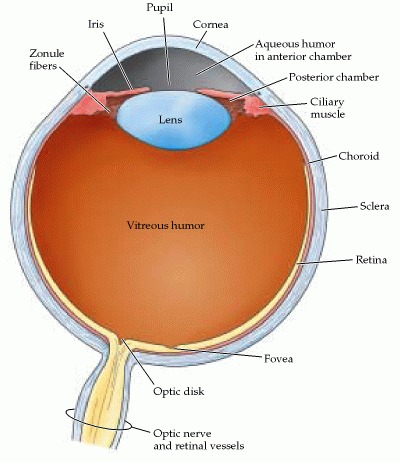
\includegraphics[width=70mm]{anatomy.jpeg}
    \caption[]{}\label{fig:}
    \end{figure}

\section{Equipamentos de Rastreamento}
Para detectar onde o participante está focando seu olhar ao longo do tempo, alguns equipamentos de ET
 fazem uso de luz infravermelha e câmeras de alta definição que projetam a luz
  diretamente no olho do participante e gravam a direção do olhar a partir do reflexo. 
  Como a luz infravermelha abrange um comprimento de onda não detectável pelo olho humano, 
  o direcionamento desta luz no olho não interfere visão do participante. 
  O cálculo do direcionamento ocular é feito com base em algoritmos próprios de cada fabricante. 
  Existem alguns tipos de equipamentos de rastreamento ocular. São eles: (1) Webcam, (2) Vestível (Werable) e (3) Baseados em Tela. 
  Webcam diz respeito a equipamentos não especializados para o uso de rastreamento; usáveis correspondem a equipamentos como óculos de rastreamento ocular 
  e realidade virtual, e os baseados em tela dizem respeito aos equipamentos de coleta especializada que podem ser acoplados a um computador Tobii Pro (2020).

  \section{Eletrooculograma} 
Fonte: https://eyewiki.aao.org/Electrooculogram

  Definition
  The electroocoulogram (EOG) is an elecrophysiologic test that measures the existing resting electrical potential between the cornea and Bruch's membrane. The mean transepithelial voltage of bovine Retinal pigment epithelium is 6 millivolts (mV). [1]
  
  History
  The EOG was described and named by Elwin Marg in 1951. Clinical applications were described first by Geoffrey Arden in 1962, who realized that the most valuable information was the comparison of the amplitudes under light and dark-adapted states (the Arden ratio).
  
  Testing process
  The patient should be dilated. The amount of light passing through the pupils is measured in a unit called Trolands (the product of luminance (cd/m2) and pupil area (mm2)).[2] Thus the pupillary diameter may change the needed luminance for the same effect on the retina.
  
  The patient should be in stable indoor lighting for at least 30 min before the test. Strong retinal illumination including retinal imaging (fluorescein angiogram, fundus photography and others) and indirect ophthalmoscopy should be avoided during this period.
  
  The patient is told to remain still other than moving his/her eyes back and forth. Four recording skin electrodes (silver-silver chloride or gold-disk) are placed at the medial and lateral canthi of both eyes, and the grounding electrode is placed on the forehead. 
  
  Principle of EOG
  The difference of electrical potential of the anterior and posterior part of the eyeball is called the standing potential.[2] Standing potential indirectly measures the transepithelial potential (TEP) of the retinal pigment epithelium (RPE). TEP is the difference of membrane potential of basolateral and apical membranes of RPE.
  
  The standing potential may be determined in 2 ways:
  
  EOG- determines function of outer retina and RPE. It has positive waveform in light and negative waveform in dark. It is recorded during 15 min of dark adaptation and 15 min of light adaptation. During 15 min of dark adaptation the standing potential usually reaches a minimum level (dark trough/DT) at 10-15 min. During 15 min of light adaptation the standing potential achieves the highest value at 7-12 min called a light peak/LP. The LP results from increased free intracellular calcium released from the endoplasmic reticulum. The role of bestrophin of endoplasmic reticulum and L type calcium channel of basolateral membrane is crucial in this. The increased intracellular calcium opens the 'Calcium dependent light peak chloride channels' of the basolateral membrane through which negative chloride ions are extruded from the RPE and the RPE depolarizes in light.[3]
  Fast Oscillations (FO)- Is an optional additional test performed using alternate 1 min dark and light periods. It has negative waveform in light and positive waveform in dark. This opposite waveform compared to EOG is related to different mechanism of FO and shorter dark and light periods. At the onset of light, there is a decrease in potassium levels at the subretinal space. This creates a strong outward hyperpolarising potassium current from the apical membrane of RPE which results in the c wave of electroretinogram. The chloride channels at the basolateral membrane (CFTR) of RPE may have important role in the generation of the FO, which may be reduced in cystic fibrosis.[4] The wave form of FO is sinusoidal compared to the EOG which has a shape of plateau after post hoc DC restoration by digital integration,
  Components of the EOG
  The light-insensitive component accounts for the dark trough and is dependent on the integrity of the retinal pigment epithelium (RPE) as well as the cornea, lens, and ciliary body. The light-sensitive component is the slow light rise of the EOG and is generated by the depolarization of the basal membrane of the RPE.
  
  Reporting of EOG
  According to the 2017 ISCEV standards,[2] the report of EOG should include
  
  Light peak: dark trough ratio (this terminology is preferred over conventional Arden ratio)
  Amplitude of dark trough (mv)
  Time from the start of light phase to light peak (when present)
  type of adapting light source
  pupil size
  Difficulties/deviation from protocol including patient compliance, inconsistent eye movements
  Interpretation of Results
  The Arden ratio, the ratio of the Light peak (Lp) to dark trough (Dt) is used to determine the normalcy of the results.
  
  An Arden ratio of 1.80 or greater is normal, 1.65 to 1.80 is subnormal, and < 1.65 is significantly subnormal.
  
  
  \subsection{Artefatos em EEG por Movimentação Ocular}

  %https://www.ncbi.nlm.nih.gov/books/NBK390358/
  \begin{figure}[h]
    \centering
    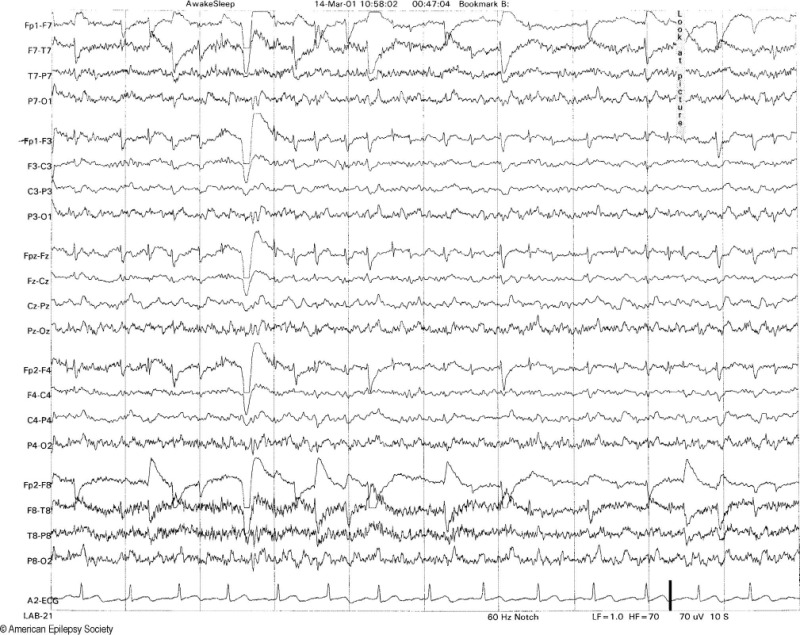
\includegraphics[width=130mm]{artefatos_oculares_EEG.jpeg}
    \caption[]{Artefatos oculares em registro de EEG. Fonte: Britton et al. (2016)}\label{fig:}
    \end{figure}

